%\documentstyle[bookman,epsf,psfig]{article}

\documentclass[12pt]{article}

\textwidth = 6.5in
\textheight = 9.05in
\topmargin 0.0in
\oddsidemargin 0.0in
\evensidemargin 0.0in

% set it so that subsubsections have numbers and they
% are displayed in the TOC (maybe hard to read, might want to disable)

\setcounter{secnumdepth}{3}
\setcounter{tocdepth}{3}

% define widow protection

\def\widow#1{\vskip #1\vbadness10000\penalty-200\vskip-#1}

% define a little section heading that doesn't go with any number

\def\littlesection#1{
\widow{2cm}
\vskip 0.5cm
\noindent{\bf #1}
\vskip 0.1cm
\noindent
}

% A paraphrase mode that makes it easy to see the stuff that shouldn't
% stay in for the final proposal

\newdimen\tmpdim
\long\def\paraphrase#1{{\parskip=0pt\hfil\break
\tmpdim=\hsize\advance\tmpdim by -15pt\noindent%
\hbox to \hsize
{\vrule\hskip 3pt\vrule\hfil\hbox to \tmpdim{\vbox{\hsize=\tmpdim
\def\par{\leavevmode\endgraf}
\obeyspaces \obeylines
\let\par=\endgraf
\bf #1}}}}}

\renewcommand{\baselinestretch}{1.2}    % must go before the begin of doc

\usepackage{graphicx}

\usepackage{url}

% go with the way that CC sets the margins

\begin{document}

% handle widows appropriately
\def\widow#1{\vskip #1\vbadness10000\penalty-200\vskip-#1}

\begin{center}

CS 112: Introduction to Computer Science II \\
Final Examination \\
%Friday, May 5, 2006 (7:00 pm) \\

\end{center}

\noindent
Answer the ten questions in this examination.  You must provide
answers to these questions on a separate sheet of paper.  Please
develop responses that clearly express your ideas in the most succinct
manner possible.  You are not permitted to complete this examination
in conjunction with any of your classmates.  Furthermore, you cannot
consult any outside references during this examination.  If you have
questions about the problems that are listed below, then please visit
my office during the examination period.  If you leave the classroom
to take the exam, you are responsible for checking the white board for
status updates.
%\newline \newline

\newpage

\begin{enumerate}

\item ({\bf 10 Points}) Answer the following questions about the basic characteristics of the Java programming language.
  For Question~\ref{encaps_example}, refer to the source code listing for {\tt BankAccount.java} that is in
  Figure~\ref{BankAccount}. For Question~\ref{values_refs}, please see the source code listing for {\tt
  ValuesAndReferences.java} in Figure~\ref{ValuesAndReferences}.

\begin{enumerate}

% \item ({\bf 2 Points}) Briefly define the terms {\em inheritance} and {\em encapsulation}. For both of these terms,
% please ensure that your response states how the Java programming language provides these features.

\item ({\bf 2 Points}) The Java language provides a class called the {\tt java.util.Scanner}.  What is the name and
  purpose of two methods that are provided by the {\tt Scanner}?

% \item \label{ctor_example} ({\bf 2 Points}) Please explain the similarities and differences between {\em instance}
%   variables and {\em static} variables.  Also, you should discuss the similarities and differences between {\em static}
%   methods and {\em instance} methods.

\item ({\bf 2 Points}) The Java language requires programmers to set the {\tt CLASSPATH} environment variable.  Please
  provide an example of the command that you would type in the terminal window to set the {\tt CLASSPATH}; your example
  should demonstrate the inclusion of both directories and JAR files in the {\tt CLASSPATH}.


\item \label{encaps_example} ({\bf 2 Points}) Both of the code
segments below deal with Java methods and instance variables. State
whether or not each of the segments would be accepted by the Java
compiler.  Provide a justification for your response.

\begin{enumerate}

\item {\tt BankAccount account1;}\\
  {\tt account1.deposit(1500);}

\item {\tt BankAccount account3 = new BankAccount();} \\
  {\tt account3.deposit(1200);} \\
  {\tt account3.deposit(account3.getBalance());}

\end{enumerate}

\item \label{values_refs} ({\bf 4 Points}) The Java programming
  language includes primitive data types like {\tt double} and objects
  like {\tt Double}.  Furthermore, it also allows for the creation of
  new classes like {\tt BankAccount} and {\tt CheckingAccount}.  Show
  what the output will be when the {\tt main} method inside of the
  {\tt ValuesAndReferences} class is executed.  Clearly state why the
  output will look the way that you suggest.

\end{enumerate}

\newpage

\item ({\bf 10 Points}) Answer the following questions about the use
  of arithmetic expressions and arrays in the Java programming
  language.

\begin{enumerate}

\item ({\bf 4 Points}) The following code segment uses arithmetic
  expressions to change the value of {\tt int} variables.  Show
  exactly what is output by the following sequence of Java statements
  (you may assume that these statements are contained within the {\tt
    main} method of an {\tt ArithmeticExpression} class):

\begin{verbatim}
        final int TRUE = 1;
        int a = 10;
        int b = 20;
        int c = TRUE;
        int d = TRUE;

        a = a + b;
        b = a - b;
        a = a - b;
        c = a % 2;
        d = b % 3;

        System.out.println(" a = "  + a + " , b = "  + b);
        System.out.println(" c = "  + c + " , d = "  + d);
\end{verbatim}

\item ({\bf 4 Points}) What are the input(s) and output(s) of a Java compiler and virtual machine?  You should answer
  this question by both writing sentences and drawing a diagram that contains meaningful labels, arrows, and boxes.

%% \item ({\bf 2 Points}) Discuss the similarities and differences
%%   between {\em instance} variables and {\em static} variables.  Also,
%%   please explain the similarities and differences between the keywords
%%   {\tt private} and {\tt protected}.

%% \item ({\bf 4 Points}) The Java programming language provides the {\tt
%%   int} and the {\tt Integer} data types.  Explain how the Java virtual
%%   machine passes parameters when a method is called.  Why can't we
%%   write a {\tt swap(int a, int b)} or {\tt swap(Integer a, Integer a)}
%%   method?  How do we write a {\tt swap} method in Java?  Your response
%%   should include Java-based pseudo-code that shows how to perform a
%%   {\tt swap} for two {\tt Objects}.

\item ({\bf 2 Points}) How do you declare and allocate an array in Java?  The Java programming language provides
facilities for {\em array bounds checking}.  What is array bounds checking? How does it work? What are its strengths and
weaknesses?

\end{enumerate}

\newpage

%% \item ({\bf 10 Points}) Computer science is about computers and
%%   computation; the essence of the discipline is the study of
%%   algorithms.  Answer the following questions about algorithms and
%%   their implementation in any programming language.

%% \begin{enumerate}

%% \item ({\bf 3 Points}) Suppose that you were asked to write a {\tt
%%   HaltingDetector} program that takes as input the source code of a
%%   Java program $P$ and an input $I$ and returns either {\tt true} or
%%   {\tt false}.  If the {\tt HaltingDetector} returns {\tt true}, this
%%   means that $P$ is guaranteed to halt on $I$.  Furthermore, if the
%%   {\tt HaltingDetector} returns {\tt false}, this means that $P$ will
%%   not halt on $I$. Explain whether or not it is possible to write the
%%   {\tt HaltingDetector} program.  Make sure that you clearly justify
%%   your response.

%% \item ({\bf 2 Points}) Suppose that you are asked to create an
%%   algorithm that will list all of the real numbers between $0.0$ and
%%   $1.0$.  Is it possible to write a pseudo-code description of an
%%   algorithm that will solve this problem?  If you answer ``yes'' you
%%   must provide the pseudo-code.  If you answer ``no'' you must state
%%   why the problem cannot be solved with an algorithm.

%% \item ({\bf 2 Points}) The are several key functions that are often
%% used to describe the performance of an algorithm.  Using a simple
%% equation, please provide an example of (i) linear, (ii) logarithmic,
%% (iii) quadratic, and (iv) exponential functions.  Your response can
%% use function $f_{i}(n)$ as the linear function, and so on for the
%% other functions.

%% \item ({\bf 3 Points}) Lothar Collatz proposed an interesting sequence
%%   of numbers that can be generated with the below steps.  State
%%   whether or not the steps that are listed below would be considered
%%   an algorithm.  Make sure that you justify your response! (Hint: to
%%   better understand these steps, choose $75$ as your arbitrary
%%   positive integer. Then, try some other positive integers as well!).

%% \begin{enumerate}

%% \item  Choose an arbitrary positive integer $A$ as the first item in the
%%         sequence. \label{step1}

%% \item  If $A = 1$ then stop. \label{step2}

%% \item  If $A$ is even, then replace $A$ by $A / 2$ and go to Step ii.
%%         \label{step3}

%% \item  If $A$ is odd, then replace $A$ by $(3 \times A) + 1$ and go to
%%         Step ii.
%%         \label{step4}

%% \end{enumerate}

%% \end{enumerate}

\newpage

\item ({\bf 10 Points}) Goodrich and Tamassia introduce the concept of
  running time and then examine the usage of empirical and analytical
  studies of a program's execution time.  Answer the following
  questions about the analysis of an algorithm's time efficiency.

\begin{enumerate}

\item ({\bf 3 Points}) Goodrich and Tamassia acknowledge that
  empirical studies of running times are quite useful.  However, these
  authors indicate that there are three major limitations to this type
  of study.  Your response to this question should clearly discuss
  each of these limitations with one or two sentences.

%% \item ({\bf 2 Points}) Suppose that you have a {\tt Hashtable} that
%%   can operate in either ``Configuration One'' or ``Configuration
%%   Two.''  Please describe the experiments that you would conduct to
%%   measure the time overhead associated with the execution of the {\tt
%%   put(k,v)} and {\tt get(k)} algorithms in both of the possible
%%   configurations.  How would you determine which configuration
%%   was better using the data produced by your experiment?

%% \item ({\bf 5 Points}) Draw a graph that illustrates the ``big-Oh''
%%   notation for the function $f(n) \in O(g(n))$.  Your graph should
%%   include the input size on the horizontal axis and the running time
%%   on the vertical axis.  Why do we use the ``big-Oh'' notation to
%%   describe the performance of an algorithm?

\item ({\bf 5 Points}) Please answer the following questions about the three methods provided by the {\tt
SortingExample} class of Figure~\ref{SortingExample}.

  \begin{enumerate}

  \item What is the input and output of the {\tt main} method?

  \item What is the worst-case time complexity of the {\tt sort} and
    {\tt print} methods?  Your response to this part of the question
    should furnish a detailed justification for the time complexity
    that you chose for each method.

  \item What kind of sorting algorithm does the {\tt sort} method
    implement?

    \item \begin{sloppypar}
      What would happen if we replaced the {\tt main} method's call to ``{\tt print(data)}'' with
      ``{\tt System.out.println(data)}'' instead?
    \end{sloppypar}

  \end{enumerate}

%% \item ({\bf 3 Points}) Complexity classes can be viewed as sets that
%%   have functions as their members.  Your answer to this question must
%%   provide three separate Venn diagrams, (i) through (iii).  Each Venn
%%   diagram must provide three different functions that are members of
%%   (i) $O(n^2)$, (ii) $\Omega(n^2)$, and (iii) $\Theta(n^2)$.
%%   Remember, in set theoretic terms, we know that $\Theta(n^2) = O(n^2)
%%   \cap \Omega(n^2)$.  Thus, the Venn diagram in (iii) should utilize
%%   the sets that you defined in (i) and (ii).

% \item ({\bf 2 Points}) Clearly explain the function $f(n)$ that
%   defines the complexity class $O(f(n))$ for the function $g(n) =
%   2^{100}$ and $g(n) \in O(f(n))$.

\item ({\bf 2 Points}) It is possible to conduct a ``doubling experiment'' to gauge the worst-case time complexity of an
algorithm. What is the complexity class (i.e., using the ``big-Oh'' notation) for the following results from a doubling
experiment?

\begin{enumerate}
    \item The algorithm's performance roughly doubles each time the problem \mbox{size doubles}.
    \item The algorithm's performance increases fourfold each time the problem \mbox{size doubles}.
\end{enumerate}

\end{enumerate}

\newpage

\item ({\bf 10 Points}) The Java programming language provides recursion
  as a construct to elegantly implement certain algorithms.  Answer the
  following questions about recursion.

\begin{enumerate}

\item ({\bf 5 Points}) Draw a diagram that explains the recursive
  calls that would occur when {\tt factorial(4)} is executed.  Make
  sure your diagram shows the input parameter and return value for
  each recursive call in a format similar to those that we created
  during class discussions.  That is, you should create a dynamic call
  tree that traces the execution of the {\tt factorial} method. Your
  response can assume that the {\tt factorial(4)} call occurs inside
  of the {\tt main(String args[])} method.

{\small
\begin{verbatim}
// pre: n is greater than or equal to zero
public static int factorial(int n)
{
  if(n == 0)
     return 1;
  else
  {
     int result = n * factorial(n - 1);
     return result;
  }
}
\end{verbatim}
}

\item ({\bf 3 Points}) A Java virtual machine (JVM) is a complex software artifact.  Using both natural language
  sentences and a diagram with labels, describe the components within a JVM.  Your response should explain how these
  different components execute a Java program.  Please make sure that you clearly discuss how the JVM handles the
  execution of programs that make recursive method calls.

  \item ({\bf 2 Points}) The \texttt{fibonacci} method below takes an input variable $n$ and returns the $n^{th}$
  Fibonacci number based on the equation $F_n = F_{n-2} + F_{n-1}$. Is this implementation efficient?  Please give
  evidence to support your assertion.

{\small \begin{verbatim}
  public static long fibonacci(int n) {
    if( n <= 1) {
      return 0;
    }
    else
      return fibonacci(n-2) + fibonacci(n-1);
  }
\end{verbatim}}

\end{enumerate}

\newpage

\item ({\bf 10 Points}) The {\tt Queue} is an abstract data type that
  adheres to the FIFO discipline.  Answer the following questions
  about the implementation and use of {\tt Queue}s.

  \begin{enumerate}

  \item ({\bf 4 Points}) What is the worst-case space complexity of an
    instance of {\tt ArrayQueue}?  What is the worst-case space
    complexity of an instance of the {\tt NodeQueue}?  Your response
    should clearly state {\em why} your selected space complexities
    are correct and explain the trade-offs associated with the {\tt
      ArrayQueue} and {\tt NodeQueue}.

  \item ({\bf 6 Points}) Draw a table that has three columns.  Label
    the first column ``Operation,'' the second column ``Output,'' and
    the third column ``front $\leftarrow Q \leftarrow$ rear.''
    Populate the second and third columns with the output and {\tt
    Queue} state, respectively, that are created by the following
    sequence of operations.  You can place one operation on a single
    row. Please make sure that you execute the operations in the order
    in which they are listed below.

    \begin{verbatim}
      1. enqueue(5), 2. enqueue(3),  3. dequeue(),   4. enqueue(7),
      5. dequeue(),  6. front(),     7. dequeue(),   8. dequeue(),
      9. isEmpty(),  10. enqueue(9), 11. enqueue(7),
      12. size(),    13. enqueue(3), 14. enqueue(5), 15. dequeue()
    \end{verbatim}

\end{enumerate}

\newpage

\item ({\bf 10 Points}) The {\tt Stack} is an ADT that adheres to the ``last in first out'' (LIFO) discipline.  Answer
the following questions about the {\tt Stack} ADT.

  \begin{enumerate}

  \item ({\bf 3 Points}) Provide a Java-based pseudo-code implementation (or, just plain pseudo-code implementation) of
    either the {\tt push} or {\tt pop} method for a simple array-based implementation of the {\tt Stack}.  You can assume
    that the {\tt Stack} is implemented with an array called {\tt S} and the top of the stack pointer is stored in an
    {\tt int} variable called {\tt t}.  Your response to this question should clearly explain the exceptions that are
    thrown by the either the {\tt push} or {\tt pop} method.

  \item ({\bf 2 Points}) The {\tt Stack} abstract data type provides methods such as {\tt isEmpty} and {\tt top}.  Using
  the ``big-Oh'' notation, what is the worst-case time complexity for each of these methods?  Please justify your chosen
  time complexities.

    \item ({\bf 5 Points}) The {\tt Stack} abstract data type can be used to determine whether or not an input {\tt
        String} of parentheses, or any other delimiting character, is either matching (e.g., ``(())'') or non-matching
      (e.g., ``((()))))'').  Using pseudo-code or Java code, please implement the {\tt isMatching\-(String s)} algorithm
      that uses a {\tt Stack} to return {\tt true} when {\tt s} is matching and {\tt false} otherwise.

  \end{enumerate}

\newpage

\item ({\bf 10 Points}) The extendable array data structure uses an
  underlying array that can ``grow'' when its space is exhausted.
  Answer these questions about this data type.

  \begin{enumerate}

  \item ({\bf 5 Points}) Clearly explain what happens when an
    extendable array is full and then the {\tt add(i,e)} method is
    invoked. Using one or more diagrams, you should discuss the four
    steps that must be taken in order to properly handle this type of
    situation.  Your response must also explain how the garbage
    collector (GC) within the Java virtual machine (JVM) is used
    during memory management.

  %% \item ({\bf 3 Points}) Identify the similarities and differences
  %%   between the {\tt java.util.Vector} and the {\tt
  %%     java.util.ArrayList}.  Your response should explain similarities
  %%   and differences related to both the performance and the
  %%   functionality of these implementations of the extendable array
  %%   ADT.

  \item ({\bf 3 Points}) What are the the similarities and differences
    between an array and the {\tt java.util.ArrayList}?  Your answer
    must identify similarities and differences in both the performance
    and the functionality of these data structures.

%%   \item ({\bf 5 Points}) Suppose that an {\tt ArrayList} called {\tt
%%     numberList} contained data values that we wanted to store on the
%%     file system.  What source code would you write to serialize and
%%     deserialize {\tt numberList} using either XStream or binary
%%     serialization with Java?  Your response to this question should
%%     include a diagram that explains the full process of serialization
%%     and deserialization.  Finally, you may assume that {\tt
%%       numberList} only contains instances of {\tt java.lang.Integer}.

  %% \item ({\bf 2 Points}) What is a {\tt java.util.Iterator}?  Your
  %%   answer should clearly discuss the steps that must be taken to
  %%   create and then use an instance of the {\tt Iterator} class.  Why
  %%   might a Java programmer who wants to print out each element in an
  %%   {\tt ArrayList} use an {\tt Iterator} instead of a {\tt for} loop?

  \item ({\bf 2 Points}) Answer the following questions about the declaration of

    {\tt
      public class ArrayIndexList<E> implements IndexList<E>}

    \begin{enumerate}

      \item What is the meaning of {\tt <E>}?

      \item Why does {\tt ArrayIndexList<E>} implement the  {\tt IndexList<E>}?

    \end{enumerate}

  \end{enumerate}

\newpage

\item ({\bf 10 Points}) The {\tt LinkedList}, {\tt DoublyLinkedList}, and {\tt Queue} are important and useful abstract
  data types (ADTs).  Answer the following questions about the design, implementation, and evaluation of these data
  types.

\begin{enumerate}

  \item ({\bf 4 Points}) Clearly explain the structure of the {\tt Node} and the {\tt DNode}.  Your response should
    indicate which of these types is used for the singly-linked list and which is used for the doubly linked list.
    Finally, your answer should include a detailed graphical depiction of the {\tt Node} and the {\tt DNode}.

  \item ({\bf 4 Points}) What are the similarities and differences between a {\tt Queue} and a {\tt DoubleEndedQueue}?
    Your response to this question should state the key methods provided by each of these data structures and then
    comment on how these methods support different types of program behavior.

  \item ({\bf 2 Points}) One way to implement a {\tt Queue} is to use an array.  Alternatively, you can implement a {\tt
      Queue} using a {\tt LinkedList}. What is the worst-case space complexity of a {\tt Queue} built with an array?
    What is the worst-case space complexity of a {\tt Queue} built with a {\tt LinkedList}? Please justify your
    response to this question.

%% \item ({\bf 4 Points}) Completely describe the operation of the {\tt
%% addFirst}, {\tt addLast}, {\tt removeFirst}, and {\tt removeLast}
%% operations for a {\tt DoubleEndedQueue} that is implemented with a
%% doubly linked list.  Your response should explain when (and if!) any
%% of these methods could throw an exception.

%%   \item \begin{sloppypar} ({\bf 5 Points}) The {\tt java.util.Vector}
%%     has a constructor that accepts two parameters in the following
%%     manner: {\tt Vector(int initialCapacity, int capacityIncrement)}.
%%     Explain the purpose of each parameter and discuss how it will
%%     impact the performance of the {\tt Vector} abstract data type.
%%     How would you conduct an experiment to quantify the influence that
%%     these two parameters have on the performance of the {\tt Vector}?
%% \end{sloppypar}


%% \item ({\bf 5 Points}) Compare and contrast the time and space
%%   overheads of a {\tt Queue} abstract data type that is implemented
%%   with either an array or a singly linked list.  Your response can
%%   refer to the {\tt Queue} that uses an array as an {\tt ArrayQueue}
%%   and the {\tt Queue} that uses a singly linked list as a {\tt
%%     NodeQueue}.

%% \item ({\bf 2 Points}) The worst-case time complexity of the {\em
%%   add(i,e)} method is given as $O(n-i+1)$ where there are $n$ elements
%%   currently stored in an array of size $N$.  Clearly explain the
%%   meaning of this time complexity and identify the worst-case values
%%   for the input parameters.  Your answer should define the variables
%%   $i$ and $e$.

%% \item \begin{sloppypar} ({\bf 4 Points}) Efficiently implement {\em
%%     remove(e)} for an input element {\em e} and the double linked
%%     list (DLL) data structure.  Your method should first find out
%%     whether or not {\em e} is contained within the DLL.  If the DLL
%%     does contain {\em e}, then your method should remove the
%%     element and then ensure that the DLL is a proper state.
%%     Element {\em e} should be returned if it was found and {\em
%%     remove} should return {\bf null} otherwise.  \end{sloppypar}

%%   \item ({\bf 3 Points}) What are the similarities and differences
%%     between the {\tt Tree} and the {\tt LinkedList}?  Your response to
%%     this question should include a representative picture of both of
%%     these data structures.

  % \item ({\bf 2 Points}) How are the {\tt Tree} and the {\tt
  %   LinkedList} similar and different?

% \item ({\bf 3 Points}) Figure~\ref{tree} furnishes an example of an
%   instance of the {\tt Tree} abstract data type.  Please provide the
%   {\em parenthetic representation} of this tree.
%
\end{enumerate}

\newpage

\item ({\bf 10 Points}) Goodrich and Tamassia claim that the {\tt
  Stack} ADT is the ``simplest of all data structures.''  The {\tt
  LinkedList} is also a valuable data structure because it provides
  additional functionality and flexibility not offered by the {\tt
    Stack}.  Answer the following questions about the methods provided
  by the {\tt Stack} and the {\tt LinkedList}.

\begin{enumerate}

\item ({\bf 5 Points}) Draw a table that has three columns.  Label the
  first column ``Operation,'' the second column ``Output,'' and the
  third column ``Stack Contents.''  Populate the second and third
  columns with the output and {\tt Stack} state, respectively, that
  are created by the following sequence of operations.  You can place
  one operation on a single row.  Make sure that you clearly indicate
  where the top of the stack is in your column that describes the
  state of the {\tt Stack}.

  \begin{verbatim}
    1. push(15),    2. push(32),
    3. pop(),       4. push(79),
    5. pop(),       6. top(),
    7. pop(),       8. pop()
  \end{verbatim}

%% \item ({\bf 2 Points}) The time complexity of the {\tt LinkedList}'s
%%   {\em get(i)} method is given as $O(min(i+1, n-i))$.  Clearly explain
%%   the meaning of this time complexity.  Finally, please identify the
%%   worst-case input parameter for the {\em get} method.  Your response
%%   should include a graphical depiction of an instance of the {\tt
%%     LinkedList} class.

\item ({\bf 3 Points}) Explain which methods of the array-based {\tt Stack} abstract data type can throw the {\tt
    EmptyStackException} and the {\tt FullStackExeption}.  Your response to this question should discuss why your
  selected methods can throw these exceptions; please also include a graphical depiction of a {\tt Stack} for each
  circumstance in which an exception can be thrown.

\item ({\bf 2 Points}) Suppose that an instance of {\tt java.util.LinkedList} contains a collection of several {\tt
    Integer} objects.  Using natural language, please describe an algorithm that can find the largest {\tt Integer}
  inside of the {\tt LinkedList}.  What is the worst-case time complexity of your implementation?  Your response should
  also furnish a diagram that helps to explain how the algorithm works.

\end{enumerate}

\newpage

\item ({\bf 10 Points}) The extendable array data structure uses an underlying array that can ``grow'' when its space is
  exhausted.  Another important data structure that often provides similar functionality is the linked list.  Answer the
  following questions about the trade-offs associated with using linked lists, arrays, and extendable arrays.

  \begin{enumerate}

%%   \item ({\bf 5 Points}) Clearly explain what happens when an
%%     extendable array is full and then the {\em add(i,e)} method is
%%     invoked. You should discuss the four steps that must be taken in
%%     order to properly handle this type of situation.  Your response
%%     must also explain how the garbage collector (GC) within the Java
%%     virtual machine (JVM) is used during memory management.

%%   \item ({\bf 6 Points}) Identify the similarities and differences
%%     between the {\tt java.util.Vector} and the {\tt
%%       java.util.ArrayList}.  Your response should explain similarities
%%     and differences related to both the performance and the
%%     functionality of these implementations of the extendable array
%%     abstract data type (ADT).

%%   \item ({\bf 2 Points}) Clearly explain the structure of the {\tt
%%     Node} and the {\tt DNode}.  Your response should indicate which of
%%     these types is used for the singly linked list and which is used
%%     for the doubly linked list.  Finally, your answer should include a
%%     simple graphical depiction of the {\tt Node} and the {\tt DNode}.

%%   \item ({\bf 2 Points}) Two important data structures include the
%%     linked list (LL) and the doubly linked list (DLL).  Please furnish
%%     a clearly labelled diagram that explains the structure of the node
%%     that makes up an LL and a DLL.

  % \item ({\bf 4 Points}) It is possible to implement a queue with
  %   either a linked list or a fixed size array.  What are the
  %   trade-offs associated with the array-based and linked list-based
  %   approaches to implementing a queue?  In your response to this
  %   question, you may use the abbreviation ``AQ'' to refer to the
  %   array-based queue and ``LLQ'' to stand for the queue that uses a
  %   linked list as its storage mechanism.

  \item ({\bf 4 Points}) Suppose that you have a properly implemented array-based queue and linked list-based queue.
    What is the worst-case time complexity of the {\tt enqueue} method for both of these queue implementations?  Your
    response to this question should include a clear justification for your chosen complexity or complexities.

  \item ({\bf 2 Points}) The array-based implementation of an extendable array performs shifting when a user executes
    the {\tt add(i,e)} and {\tt remove(i)} methods.  Why do both of these methods shift data values in the array?  In
    which direction do the {\tt add} and {\tt remove} methods respectively shift the data values?

  \item ({\bf 4 Points}) The {\tt main} method in Figure~\ref{Queue}'s {\tt QueueDiscipline} class constructs an
    instance of the {\tt java.util.concurrent.ArrayBlockingQueue} and then performs several operations on this instance.
    What is the output of the {\tt main} method?

%% \item ({\bf 4 Points}) Sketch the implementation of either the {\em
%%     add(i,e)} or {\em remove(i)} method that is part of a simple
%%     array-based implementation of an extendable array.  Your sketch
%%     should clearly explain how to perform the shifting of array
%%     elements.  The parameter $i$ denotes the index subject to addition
%%     or removal and the parameter $e$ represents the data element that
%%     must be added.

%%   \item ({\bf 2 Points}) Suppose that we were interested in storing an
%%     instance of an extendable array on the file system.  Explain how
%%     we could use a Java serialization primitive to perform this
%%     operation.  What is the difference between the XStream serialization
%%     primitive and the traditional Java serialization primitive?

  \end{enumerate}

%% \item ({\bf 10 Points}) The {\tt Tree} is an important and interesting
%%   data structure that is used in file systems, databases, and a host
%%   of other real world software applications.

%% \begin{enumerate}

%% \item ({\bf 2 Points}) The {\tt SuffixTree} is a data structure that
%%   supports the efficient identification of the longest common
%%   substring (LCS).  The R programming language contains an interface
%%   to the {\tt libstree} library available from
%%   \url{http://www.icir.org/christian/libstree/}.  Please provide the
%%   output for each of the following calls to {\tt
%%     getLongestCommonSubstring}.

%%   \begin{enumerate}

%%   \item \begin{verbatim}
%%   otherExampleStrings = c("examples", "example", "examination")
%%   getLongestCommonSubstring(otherExampleStrings)
%%   \end{verbatim}

%%   \item \begin{verbatim}
%%   otherWikipediaExample = c("BABA", "ABBA")
%%   getLongestCommonSubstring(otherWikipediaExample)
%%   \end{verbatim}

%%   \end{enumerate}

%% \item ({\bf 3 Points}) The figure below contains an example of a tree.
%%   For this part of the question, please give a complete listing of the
%%   root(s) and external node(s) of this tree.  When you are responding
%%   to this question, you should remember that the terms ``external
%%   node'' and ``leaf'' have the same meaning.

%% %% \item ({\bf 5 Points}) Please produce a parenthetic representation for
%% %%   the example tree data structure.  In response to this question, you
%% %%   should explain the meaning of each syntactic element of the
%% %%   parenthetic representation (i.e., ``('', ``)'', and ``,'').

%% \item ({\bf 5 Points}) What is the depth of the following nodes -- A,
%%   X, R, I, Z?  What is the height of this tree?  In your response to
%%   this question, you should intuitively explain how to calculate the
%%   height of a {\tt Tree}.

%% \end{enumerate}

%% \begin{figure}[h]

%%   \begin{center}
%%   \includegraphics[totalheight=0.3\textheight]{dct_tcm_tree_bw.ps}
%%   \end{center}

%%   \vspace*{-.2in}

%%   \caption{An Example of a Tree Data Structure.}

%% \end{figure}

\newpage

\begin{figure}[t]

\footnotesize{
\begin{verbatim}
public class BankAccount
{

  private double balance;

  public BankAccount()
  {

    balance = 0;

  }

  public BankAccount(double initialBalance)
  {

    balance = initialBalance;

  }

  public void deposit(double amount)
  {

    balance = balance + amount;

  }

  public void withdraw(double amount)
  {

    balance = balance - amount;

  }

  public double getBalance()
  {

    return balance;

  }

}
\end{verbatim}
}
\caption{The {\tt BankAccount} Class.}
\label{BankAccount}
\end{figure}

\begin{figure}[t]

\footnotesize{
\begin{verbatim}
public class ValuesAndReferences
{

  public static void main(String[] args)
  {

    double balance1 = 1000;
    double balance2 = balance1;
    balance2 = balance2 + 500;

    BankAccount account1 = new BankAccount(1000);
    BankAccount account2 = account1;
    account2.deposit(500);

    BankAccount account3 = new BankAccount(1000);
    BankAccount account4 = new BankAccount(account3.getBalance());
    account4.deposit(500);

    System.out.println(" balance1: " + balance1);
    System.out.println(" balance2: " + balance2);
    System.out.println();

    System.out.println(" account1 balance: " + account1.getBalance());
    System.out.println(" account2 balance: " + account2.getBalance());
    System.out.println();

    System.out.println(" account3 balance: " + account3.getBalance());
    System.out.println(" account4 balance: " + account4.getBalance());
    System.out.println();

  }

}
\end{verbatim}
}

\caption{The {\tt ValuesAndReferences} Class.}
\label{ValuesAndReferences}
\end{figure}

\begin{figure}[t]

\footnotesize{
\begin{verbatim}
public class SortingExample
{
    public static void main(String[] args)
    {
        int[] data = {45, 5, 0, 10, 19, 72, 6, 88, 4, 999};
        print(data);
        sort(data);
        print(data);
    }

    public static void print(int array[])
    {
        int i = 0;
        for(i=0; i < array.length; i++)
            {
                System.out.print(array[i] + "  " );
            }
        System.out.println();
        System.out.println();
    }

    public static void sort(int[] data)
    {
        for (int k = 0; k < data.length - 1; k++)
            {
                boolean isSorted = true;
                for (int i = 1; i < data.length - k; i++)
                    {
                        if (data[i] < data[i - 1])
                            {
                                int tempVariable = data[i];
                                data[i] = data[i - 1];
                                data[i - 1] = tempVariable;
                                isSorted = false;
                            }
                    }
                if (isSorted)
                    break;
            }
    }
}
\end{verbatim}
}

\caption{The {\tt SortingExample} Class.}
\label{SortingExample}
\end{figure}

% \newpage
%
% \begin{figure}[h]
%
%   \begin{center}
%   \includegraphics[totalheight=0.75\textheight]{filesystem-tree.pdf}
%   \end{center}
%
%   \vspace*{-.2in}
%
%   \caption{An Example of a Tree Data Structure.}
%   \label{tree}
%
% \end{figure}

\newpage

\begin{figure}[t]

\footnotesize{
\begin{verbatim}
import java.util.concurrent.ArrayBlockingQueue;

public class QueueDiscipline
{

    public static void main(String[] args)
    {

        ArrayBlockingQueue queue = new ArrayBlockingQueue(10);

        System.out.println(" Input phase ... " );
        for(int i = 0; i < 10; i++)	    {

                Integer value = new Integer(i);
                queue.offer(value); // run an "enqueue" method call
                System.out.println(value);

        }

        System.out.println(" State of the Queue: " + queue.toString());

        System.out.println(" Output phase ... " );
        while(queue.peek() != null) {

                Integer value = (Integer)queue.remove(); // run a "dequeue" method call
                System.out.println(value);

        }

        System.out.println(" State of the Queue: " + queue.toString());

    }

}
\end{verbatim}
}

\caption{The {\tt QueueDiscipline} Class.}
\label{Queue}
\end{figure}

%% \begin{figure}[t]

%% \begin{verbatim}
%% public static <E> int depth (Tree<E> T, Position<E> v) {
%%     if (T.isRoot(v))
%%       return 0;
%%     else
%%       return 1 + depth(T, T.parent(v));
%%   }
%% \end{verbatim}
%% \caption{The {\tt depth} Method for a {\tt Tree}.}
%% \label{fig:depth}
%% \end{figure}

%% \begin{figure}[t]

%% \begin{verbatim}
%%    public static <E> int height1 (Tree<E> T) {
%%      int h = 0;
%%      for (Position<E> v : T.positions()) {
%%        if (T.isExternal(v))
%%          h = Math.max(h, depth(T, v));
%%      }
%%      return h;
%%    }
%% \end{verbatim}
%% \caption{The {\tt height1} Method for a {\tt Tree}.}
%% \label{fig:height1}
%% \end{figure}

%% \begin{figure}

%% \begin{verbatim}
%%   public static <E> int height2 (Tree<E> T, Position<E> v) {
%%     if (T.isExternal(v)) return 0;
%%     int h = 0;
%%     for (Position<E> w : T.children(v))
%%       h = Math.max(h, height2(T, w));
%%     return 1 + h;
%%   }
%% \end{verbatim}
%% \caption{The {\tt height2} Method for a {\tt Tree}.}
%% \label{fig:height2}
%% \end{figure}

\end{enumerate}

\end{document}



